\section{Evaluation}\label{sec:evaluation}

\subsection{Evidence Layers and Reporting Policy}

The evaluation is intentionally split into two layers.

\textbf{Public layer.} This layer is already available in the repository and is therefore used as the current evidence base for this draft. It consists of a 32-sample balanced corpus derived from OWASP Benchmark v1.2~\cite{owaspBenchmark2026}, covering four request families: SQL injection, cross-site scripting, path traversal, and command injection. The repository evaluation compares three configurations: \texttt{single\_agent}, \texttt{multi\_agent\_no\_debate}, and \texttt{multi\_agent\_with\_debate}.

\textbf{Private layer.} This layer is reserved for future labeled alert data. The present manuscript specifies how such a layer should be reported, but does not fabricate its results. If timestamps are available, splitting should follow early 70\%, middle 10\% for threshold calibration, and late 20\% for final reporting. Otherwise, a fixed-seed stratified 80/20 split should be used.

\subsection{Metrics}

The public layer reports the metrics that directly test the thesis of the paper:
\begin{itemize}
  \item accuracy, precision, recall, and F1;
  \item false positive count and false negative count;
  \item debate trigger ratio and average debate rounds;
  \item end-to-end orchestration latency.
\end{itemize}
The emphasis is deliberate. Since the paper claims that debate helps on ambiguous cases, false positives and debate trigger behavior are treated as first-class outputs rather than footnotes.

\subsection{Public Baseline Comparison}

Table~\ref{tab:public-baselines} reports the main public comparison. The result is compact but important. The debate-enabled setting eliminates the four false positives that remain in both non-debate baselines, improving accuracy from 87.5\% to 100\% on the current balanced slice. The repository summary further notes that these four false positives all occur in benign command-injection-like requests, which is exactly the kind of ambiguity this method is meant to resolve.

\begin{table*}[t]
  \centering
  \footnotesize
  \caption{Public baseline comparison on the repository OWASP-derived 32-sample corpus.}
  \label{tab:public-baselines}
  \setlength{\tabcolsep}{5pt}
  \begin{tabularx}{\textwidth}{@{}lcccccc@{}}
    \toprule
    Configuration & Accuracy & Precision & Recall & F1 & False positives & False negatives \\
    \midrule
    \texttt{single\_agent} & 0.8750 & 0.8000 & 1.0000 & 0.8889 & 4 & 0 \\
    \texttt{multi\_agent\_no\_debate} & 0.8750 & 0.8000 & 1.0000 & 0.8889 & 4 & 0 \\
    \texttt{multi\_agent\_with\_debate} & 1.0000 & 1.0000 & 1.0000 & 1.0000 & 0 & 0 \\
    \bottomrule
  \end{tabularx}
\end{table*}

In this comparison, \texttt{single\_agent} uses the repository's \texttt{cloud\_only} route, while \texttt{multi\_agent\_no\_debate} preserves the role decomposition but disables explicit disagreement handling. The paper's main claim should not be overstated beyond this result. The corpus is small, balanced, and derived from a benchmark suite rather than from production traffic. Still, the pattern is coherent with the method: debate is most useful when a superficially suspicious request is actually benign.

\subsection{Ablation and Overhead}

Table~\ref{tab:ablation} combines the evidence currently available for ablation-style interpretation. The first part isolates the effect of debate. The second part reports route-mode latency observations from the repository summary. These values are orchestration measurements and should not be interpreted as full model inference latency. The third part records the current system-overhead snapshot from the validated workspace report.

\begin{table*}[t]
  \centering
  \footnotesize
  \caption{Repository-traceable ablation and overhead evidence.}
  \label{tab:ablation}
  \setlength{\tabcolsep}{5pt}
  \begin{tabularx}{\textwidth}{@{}p{0.18\textwidth}p{0.18\textwidth}p{0.20\textwidth}Y@{}}
    \toprule
    Evidence slice & Setting & Observed metric & Interpretation \\
    \midrule
    Debate ablation & no debate & accuracy 0.8750; 4 false positives & retains all four benign command-injection-like false positives \\
    Debate ablation & with debate & accuracy 1.0000; mean orchestration latency 0.5000 ms & removes all four false positives on the public slice \\
    Route mode & \texttt{cloud\_only} & mean orchestration latency 0.8438 ms & highest observed orchestration overhead in the repository summary \\
    Route mode & \texttt{local\_preferred} & mean orchestration latency 0.7500 ms & lower orchestration overhead than \texttt{cloud\_only} \\
    Route mode & \texttt{hybrid\_verify} & mean orchestration latency 0.7813 ms; debate latency 0.0938 ms & lowest reported debate latency among the route-mode entries \\
    Workspace smoke benchmark & fastpath snapshot & 1329.79 QPS; 21 ms p95 latency & validated smoke profile only, not a full production-scale claim \\
    \bottomrule
  \end{tabularx}
\end{table*}

Across the public corpus, debate is triggered on 12 out of 32 requests, or 37.5\%, with an average of 0.75 debate rounds per sample. This is consistent with the intended design: most requests do not require explicit disagreement handling, while a smaller subset benefits from it.

\subsection{Limitations of the Current Public Layer}

The public evidence should be read with several constraints in mind. First, the corpus size is too small for broad generalization. Second, a benchmark-derived slice is not equivalent to operational traffic. Third, the repository includes a scaffold for a ModSecurity + CRS baseline, but it was not executable in the current environment and is therefore not reported as a competitive result. The comparison is mentioned only to document evaluation intent and to avoid implying that the baseline already ran~\cite{owaspCRS2026}.

\begin{figure}[t]
  \centering
  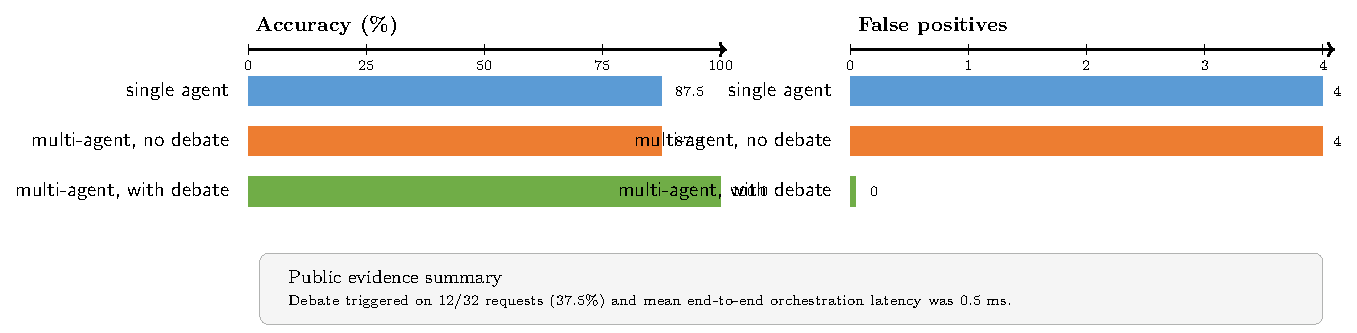
\includegraphics[width=\linewidth]{fig-results-summary.pdf}
  \caption{Summary of the public benchmark and overhead evidence used in this draft.}
  \label{fig:results-summary}
\end{figure}

\subsection{Private Labeled-Alert Reporting Template}

The manuscript reserves a second evidence layer for private labeled alerts because that is the correct place to test whether debate reduces false positives on real ambiguity. Table~\ref{tab:private-template} provides the reporting template instead of inventing numbers.

\begin{table}[t]
  \centering
  \caption{Template for the private labeled-alert dataset revision.}
  \label{tab:private-template}
  \footnotesize
  \begin{tabularx}{\columnwidth}{@{}p{0.39\columnwidth}Y@{}}
    \toprule
    Field & Value to report later \\
    \midrule
    Total labeled alerts & TBD \\
    Distinct protected applications & TBD \\
    Label space & benign / suspicious / malicious or mapped binary labels \\
    Time span covered & TBD \\
    Split policy & 70/10/20 by time if timestamps exist, else fixed-seed stratified 80/20 \\
    Main thesis test & whether debate reduces false positives on ambiguous alerts \\
    Required baselines & single agent, multi-agent without debate, multi-agent with debate \\
    Required error analysis & at least 10 representative false positives before and after debate \\
    \bottomrule
  \end{tabularx}
\end{table}

This template keeps the draft honest: the paper is ready for a stronger second evidence layer, but it does not pretend that the layer already exists.
